\section{Architecture}
This section explains the overall architecture of the Google+ search engine and mentions used APIs and libraries.
\subsection*{Overall architecture}
\begin{figure}[h]
\begin{center}
    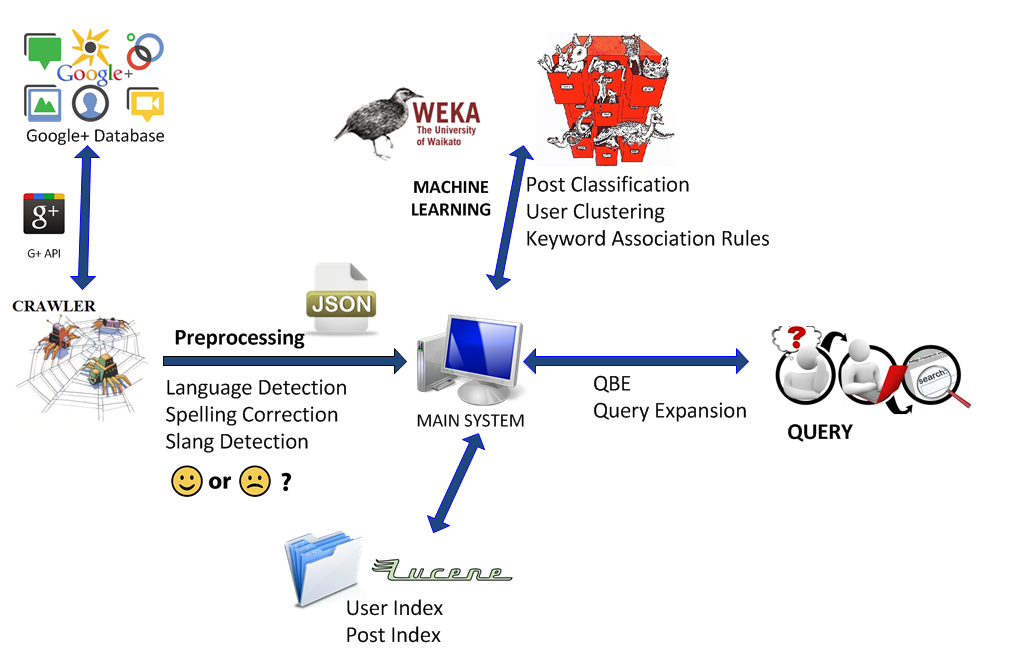
\includegraphics[scale=0.4]{images/architecture.png}
	\caption{Architecture sketch\label{architecture_sketch}}
\end{center}
\end{figure}
The architecture of the systems consist of a crawler that will get data from the Google+ database using the Google+ API. The output from the crawler is preprocessed with language and slang detection, spelling correction, and sentiment analysis. Preprocessed data is then used for machine learning, pattern mining and index building. The machine learning tasks consist of the training of classifiers and the clustering of user profiles. The queries can be processed with additional query by example and query expansion techniques.
\subsection*{Used API and Tools}
\subsubsection*{WEKA}
WEKA is an open source suite of machine learning algorithms. It contains tools for preprocessing, classification, clustering and other data mining related tasks. 
\subsubsection*{Apache Lucene}
Apache Lucene is an open source project, high performance, fully-featured text search engine library in Java. It includes an indexing and searching library that is suitable for making  a simple search engine.
\subsubsection*{Google+ API}
For the training and testing of our classifiers and for building a search engine, which can be queried by users, a large amount of data was required. To retrieve this data we used the Google+ Application Programmable Interface (API). This interface allows querying for Google+ posts and user profiles via web requests and returns an easy to parse result. The API is still under development by Google, and this provided some inconsistencies between the API specification and the results retrieved from our queries.
\subsubsection*{NLTK}
NLTK is a widely used library in the domain of human language processing which is written in Python. It can perform most of the operations one might need when working with a natural language, from sentence splitting to text classification. 
\subsubsection*{Alchemy API}
AlchemyAPI provides cloud-based text analysis infrastructure which can be used for various NLP related task. We used AlchemyAPI to extract the keywords from user posts, which are then used in keyword pattern mining. 
\subsubsection*{OpenNLP}
OpenNLP is a Java library for machine learning and processing of a text written in a natural language. For this task, it was used for tokenization and part-of-speech tagging.